\documentclass[aps,prb,onecolumn,nofootinbib,superscriptaddress]{revtex4-2}
\usepackage{amsmath,amssymb,amsthm,mathtools,bm}
\usepackage{booktabs}
\usepackage{tikz}
\usetikzlibrary{arrows.meta,calc,positioning}
\usepackage[colorlinks=true,linkcolor=blue,citecolor=blue,urlcolor=blue]{hyperref}
\usepackage{microtype}
\newcommand{\One}{\hat{\mathbf{1}}}
\newcommand{\Tr}{\operatorname{Tr}}
\newcommand{\fSWAP}{\operatorname{fSWAP}}
\newcommand{\ket}[1]{\lvert #1\rangle}
\newcommand{\braket}[2]{\langle #1\vert #2\rangle}
\newcommand{\Abar}{\overline A}
\hypersetup{pdftitle={Entangling Capacity of a Local Adaptive Fermion Circuit},
pdfauthor={Class-A Fermionic Adaptive-Circuit Project}}
\begin{document}
\title{Entangling Capacity of a Local Adaptive Fermion Circuit}
\author{Class-A Fermionic Adaptive-Circuit Project}
\noaffiliation
\date{October 6, 2026}
\begin{abstract}
We explain how locality constrains entanglement production in a fermionic
circuit with measurements and outcome-dependent feedback. Starting from a
single conditional trajectory, we derive a bound on Schmidt-rank growth and
then convert it into a physical-depth bound. We specialize the argument to
occupation measurements of finite-range overcomplete Wannier modes followed
by fresh-ancilla fermionic-swap correction, deriving the conditional
operators and their cut-crossing ranks explicitly. For a strip intersecting
two critical interfaces in a two-dimensional system, product-state
preparation and conformal entropy scaling imply the necessary resource
$D_{\mathrm{circ}}N_x=\Omega(\log N_y)$. This is a restriction on
preparation, not a proof of criticality or a prediction for convergence time.
\end{abstract}
\maketitle
\setcounter{tocdepth}{2}
\tableofcontents

\section{Conditional dynamics and entanglement across a cut}
\label{sec:conditional}
Measurements and classical feedback can prepare correlations in ways that a
local unitary circuit cannot. Nevertheless, a bounded quantum operation
does not acquire unlimited capacity to create entanglement across a spatial
cut. The quantity appropriate to a bound valid for each measurement branch
is the logarithm of Schmidt rank. We develop this argument following
Appendix D of Lu, Lessa, Kim, and Hsieh \cite{LuLessaKimHsieh2022}, then
specialize it to the fermionic controller motivated by Bhuiyan, Pan, and
Jian (BPJ) \cite{BhuiyanPanJian2026}.

For a pure input, a measurement with outcome $m$ is specified by a Kraus
operator $\hat K_m$ and a nonnegative weight $w_m$. The
positive-operator-valued measure (POVM) condition and Born probability are
\begin{equation}
 \sum_m w_m\hat K_m^\dagger\hat K_m=\One,\qquad
 p_m=w_m\braket{\psi}{\hat K_m^\dagger\hat K_m\psi}.
 \label{eq:povm}
\end{equation}
We subsequently absorb $\sqrt{w_m}$ into the branch operator; this scalar
does not change its rank. Outcome-dependent unitary feedback is also
included in that operator. For a full record $\boldsymbol m=(m_1,\ldots,m_M)$,
the many-body evolution operator (mEO) and normalized branch are
\begin{align}
 \hat V_{\boldsymbol m}
 &=\hat O_{m_M}(\boldsymbol m_{<M})\cdots\hat O_{m_2}(m_1)\hat O_{m_1},
 \label{eq:branch-word}\\
 p_{\boldsymbol m}
 &=\|\hat V_{\boldsymbol m}\ket{\psi_{\mathrm{in}}}\|^2,\qquad
 \ket{\psi_{\boldsymbol m}}
 =\frac{\hat V_{\boldsymbol m}\ket{\psi_{\mathrm{in}}}}
 {\sqrt{p_{\boldsymbol m}}},\quad p_{\boldsymbol m}>0.
 \label{eq:normalized-branch}
\end{align}
The rightmost factor acts first. Earlier outcomes may determine both the
kind and location of a later operation. Fixing a record is a mathematical
conditioning, not a prescription to postselect it experimentally.

Choose a spatial bipartition $A\cup\Abar$ and a fermionic mode ordering
adapted to it. Here $A$ denotes a region, not the ancillary system; ancillary
quantities carry the subscript $\mathrm a$. A graded Fock-space
factorization can be represented by an ordinary tensor product with
explicit parity strings. Physical branch operators are taken to have
definite fermion parity, as do all operators in the controller below;
physical pure input states have definite total parity. In that
representation, the Schmidt decomposition is
\begin{equation}
 \ket{\psi}=\sum_{i=1}^{\chi_A}\sqrt{p_i}\,
 \ket{\phi_i}_A\otimes\ket{\theta_i}_{\Abar},
 \qquad p_i>0,\quad\sum_i p_i=1.
 \label{eq:schmidt}
\end{equation}
Both vector sets are orthonormal, and the reduced density operator has
exactly $\chi_A$ nonzero eigenvalues. With natural logarithms,
\begin{equation}
 S_0(A)=\log\chi_A,\qquad
 S_q(A)=\frac{\log\sum_i p_i^q}{1-q},\qquad
 S_1(A)=-\sum_i p_i\log p_i .
 \label{eq:entropies}
\end{equation}
The Hartley entropy $S_0$ counts components regardless of their weights.
The von Neumann entropy is the continuous $q\to1$ limit; for all $q>0$,
$S_q\leq S_0$.

\subsection{Why von Neumann entropy growth is different}
A local filter cannot create independent Schmidt components, but it can
change their relative probabilities. Put a flag mode $f$ in $A$ and consider
\begin{equation}
 \ket{\Psi}=\sqrt{1-\epsilon}\ket{0}_f
 \ket{a_0}_{A'}\ket{b_0}_{\Abar}
 +\sqrt{\epsilon}\ket{1}_f\ket{\Phi_L}_{A'\Abar},
 \qquad A=f\cup A'.
 \label{eq:filter-example}
\end{equation}
Choose $S_1(\Phi_L)=\Theta(L)$ and the $\Abar$ Schmidt support of
$\Phi_L$ orthogonal to $\ket{b_0}$. The reduced eigenvalues are
$1-\epsilon$ and $\epsilon$ times those of $\hat\rho_{A'}^{\Phi_L}$, hence
\begin{equation}
 S_1(A;\Psi)=H_2(\epsilon)+\epsilon S_1(A';\Phi_L),\qquad
 H_2(\epsilon)=-\epsilon\log\epsilon-(1-\epsilon)\log(1-\epsilon).
 \label{eq:filter-entropy}
\end{equation}
For $\epsilon=O(L^{-1})$, the input entropy is $O(1)$. Measuring the flag
and obtaining $1$ leaves entropy $\Theta(L)$, even though the operation is
entirely in $A$. The two components can be chosen in the same total
fermion-parity sector, so the example needs no parity-violating measurement.

The initial Schmidt rank was already $1+\chi_A(\Phi_L)$. There is no
increase in $S_0$. Thus a branchwise bound on $\Delta S_0$ is not a bound
on $\Delta S_1$. For a product input, however, $S_0^{\mathrm{in}}=0$,
and bounding $S_0^{\mathrm{out}}$ bounds every $S_q^{\mathrm{out}}$.

\section{Capacity of an individual conditional operation}
\label{sec:rank}
Across the same bipartition, expand an operation as
\begin{equation}
 \hat O=\sum_{\alpha=1}^{r}\sigma_\alpha
 \hat O^A_\alpha\otimes\hat O^{\Abar}_\alpha .
 \label{eq:operator-schmidt}
\end{equation}
The smallest number of terms is the operator-Schmidt rank $r$. Equivalently,
reshape the matrix elements so that the input/output indices on $A$ form
one index and those on $\Abar$ form the other; the rank of this reshaped
matrix is $r$. Any explicit product expansion supplies an upper bound.

Applying Eq.~\eqref{eq:operator-schmidt} to Eq.~\eqref{eq:schmidt} gives
\begin{equation}
 \hat O\ket{\psi}
 =\sum_{\alpha=1}^{r}\sum_{i=1}^{\chi_A}
 \sigma_\alpha\sqrt{p_i}\,
 \bigl(\hat O^A_\alpha\ket{\phi_i}_A\bigr)\otimes
 \bigl(\hat O^{\Abar}_\alpha\ket{\theta_i}_{\Abar}\bigr).
 \label{eq:rank-product}
\end{equation}
The output is a sum of at most $r\chi_A$ product vectors. They need not
be orthogonal or independent, so its Schmidt rank is at most this number.
Normalization multiplies the coefficient matrix by a scalar. Therefore
\begin{equation}
 \chi_A^{\mathrm{out}}\leq r\chi_A^{\mathrm{in}},\qquad
 S_0^{\mathrm{out}}-S_0^{\mathrm{in}}\leq\log r .
 \label{eq:one-step}
\end{equation}
No inverse is used: singular projectors are allowed. Zero-norm branches
are excluded only because they cannot be normalized.

An operation supported on one side has a one-term product representation.
For an odd fermionic operator on $\Abar$, its representation contains a
parity factor on $A$; it is still one product term. The relevant support
is physical fermionic support, not the apparent length of a parity string.

Let $\mathcal C_\partial(\boldsymbol m)$ contain the operations whose
physical supports cross the cut on a realized record. Iteration gives
\begin{align}
 \chi_A(\psi_{\boldsymbol m})
 &\leq\chi_A(\psi_{\mathrm{in}})
 \prod_{j\in\mathcal C_\partial(\boldsymbol m)}r_j,\\
 S_0(A;\psi_{\boldsymbol m})-S_0(A;\psi_{\mathrm{in}})
 &\leq\sum_{j\in\mathcal C_\partial(\boldsymbol m)}\log r_j .
 \label{eq:exact-bound}
\end{align}
Feedback changes the realized sequence but not the proof for that sequence.
This bound needs no minimum outcome probability, Gaussianity, translation
invariance, or invertibility.

\section{From crossing operations to physical circuit depth}
\label{sec:depth}
Suppose each operation has support diameter at most $R$, onsite Hilbert
spaces have dimension $d_{\mathrm{loc}}$, and the lattice has bounded
coordination. Fix $R$ and $d_{\mathrm{loc}}$ as the system grows. A
physical layer contains mutually nonoverlapping quantum operations.
A crossing gate meeting $s_A$ sites in $A$ and $s_{\Abar}$ in $\Abar$ has
\begin{equation}
 r_j\leq\min\{d_{\mathrm{loc}}^{2s_A},
                   d_{\mathrm{loc}}^{2s_{\Abar}}\}\leq r_*,
 \label{eq:local-rank}
\end{equation}
because these are its two local operator-space dimensions. For fixed
range, $r_*$ is size independent.

Crossing gates meet the boundary neighborhood of thickness $R$, whose
volume on a regular lattice is bounded by a constant times $|\partial A|$.
Nonoverlap limits their number per layer to
$\nu_\partial|\partial A|$, where $\nu_\partial$ is size independent.
For $D_{\mathrm{circ}}$ layers,
\begin{equation}
 \Delta S_0(A)\leq D_{\mathrm{circ}}\nu_\partial|\partial A|\log r_*
 =\kappa D_{\mathrm{circ}}|\partial A|.
 \label{eq:depth-bound}
\end{equation}
This is the entanglement-growth bound of Ref.~\cite{LuLessaKimHsieh2022},
Appendix D. For pure product inputs it implies
\begin{equation}
 S_q^{\mathrm{out}}(A)\leq\kappa D_{\mathrm{circ}}|\partial A|,
 \qquad q>0.
 \label{eq:renyi-bound}
\end{equation}

Local product ancillas add no initial cross-cut rank. A fixed ancillary
overhead is absorbed in $d_{\mathrm{loc}}$ and $\kappa$. If an entangled
ancilla is discarded without a resolved outcome, the physical output can
be mixed: one must specify a purification and its cut before using the
pure-state argument. The controller below instead leaves its outgoing
ancilla factorized on every record.

Physical depth is not a simulation update count. Overlapping OW
measurements in one sweep cannot all count as one quantum layer.
Bounded-support patches admit a finite coloring, but reordering
noncommuting measurements can change the protocol; a coloring alone does
not establish the depth of the original ordered sweep. Classical
communication can be nonlocal in this bound. Including its physical
latency adds a time cost without weakening the rank inequality.

\begin{figure}[tb]
\centering
\begin{minipage}{0.47\textwidth}
\centering
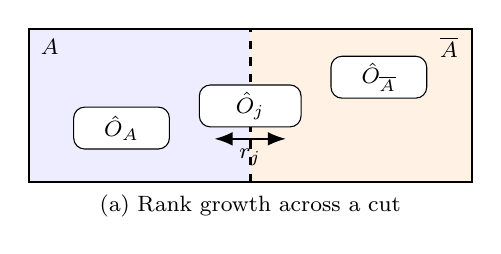
\begin{tikzpicture}[x=0.76cm,y=0.76cm,>=Latex,font=\footnotesize]
 \fill[blue!7] (0,0) rectangle (3.7,2.55);
 \fill[orange!10] (3.7,0) rectangle (7.4,2.55);
 \draw[thick] (0,0) rectangle (7.4,2.55);
 \draw[very thick,dashed] (3.7,0) -- (3.7,2.55);
 \node at (0.35,2.25) {$A$};
 \node at (7.02,2.25) {$\Abar$};
 \draw[rounded corners,fill=white] (0.75,0.55) rectangle (2.35,1.25);
 \node at (1.55,0.90) {$\hat O_A$};
 \draw[rounded corners,fill=white] (5.05,1.40) rectangle (6.65,2.10);
 \node at (5.85,1.75) {$\hat O_{\Abar}$};
 \draw[rounded corners,fill=white] (2.85,0.92) rectangle (4.55,1.62);
 \node at (3.70,1.27) {$\hat O_j$};
 \draw[<->,thick] (3.10,0.72) -- node[below] {$r_j$} (4.30,0.72);
 \node at (3.7,-0.40) {(a) Rank growth across a cut};
\end{tikzpicture}
\end{minipage}
\hfill
\begin{minipage}{0.49\textwidth}
\centering
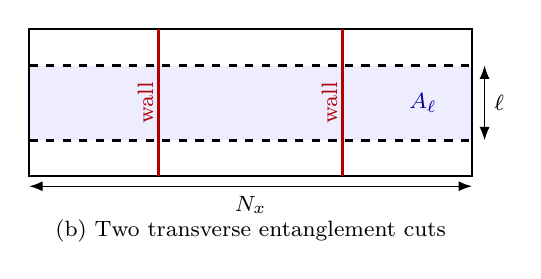
\begin{tikzpicture}[x=0.73cm,y=0.73cm,>=Latex,font=\footnotesize]
 \fill[blue!7] (0,0.62) rectangle (7.7,1.92);
 \draw[thick] (0,0) rectangle (7.7,2.55);
 \draw[very thick,dashed] (0,0.62) -- (7.7,0.62);
 \draw[very thick,dashed] (0,1.92) -- (7.7,1.92);
 \draw[very thick,red!70!black] (2.25,0) -- (2.25,2.55);
 \draw[very thick,red!70!black] (5.45,0) -- (5.45,2.55);
 \node[blue!60!black] at (6.85,1.27) {$A_\ell$};
 \node[red!70!black,rotate=90] at (2.02,1.27) {wall};
 \node[red!70!black,rotate=90] at (5.22,1.27) {wall};
 \draw[<->] (0,-0.18) -- node[below] {$N_x$} (7.7,-0.18);
 \draw[<->] (7.92,0.62) -- node[right] {$\ell$} (7.92,1.92);
 \node at (3.85,-0.95) {(b) Two transverse entanglement cuts};
\end{tikzpicture}
\end{minipage}
\caption{(a) Only cut-crossing operations can increase Schmidt rank; a
crossing operation of operator-Schmidt rank $r_j$ multiplies it by at most
$r_j$. (b) A full-width strip on a torus has two cuts of length $N_x$.
Localization near the walls does not reduce the subsystem boundary to two
points. Opposite edges of the rectangle are periodically identified.}
\label{fig:cuts}
\end{figure}

\section{Occupation measurements with fermionic-swap correction}
\label{sec:fermionic}
\subsection{The four conditional operators}
Consider one normalized overcomplete Wannier (OW) mode in BPJ's
fill-lower-band, deplete-upper-band construction \cite{BhuiyanPanJian2026}.
Suppressing its position, family, and band labels, write
\begin{equation}
 \hat\chi=\sum_{x\in X}\chi_x\hat c_x,\qquad
 \sum_{x\in X}|\chi_x|^2=1,\qquad
 \{\hat c_x^\dagger,\hat c_y\}=\delta_{xy}.
 \label{eq:ow}
\end{equation}
The index $x$ includes orbitals. The patch $X$ is obtained by finite-range
truncation and renormalization. Distinct OW modes are generally
nonorthogonal, so their number operators need not commute. Only the
single-mode algebra is used in the following step. Define
\begin{equation}
 \hat N_\chi=\hat\chi^\dagger\hat\chi,\qquad
 \hat\Pi_1=\hat N_\chi,\qquad
 \hat\Pi_0=\One-\hat N_\chi.
 \label{eq:projectors}
\end{equation}
The relations $\hat\chi^2=0$ and
$\hat\chi\hat\chi^\dagger=\One-\hat N_\chi$ imply
$\hat N_\chi^2=\hat N_\chi$, so these are complementary projectors.

The target is $s=1$ for filling and $s=0$ for depletion. Measure $m$ and
do nothing when $m=s$. For a mismatch, supply a fresh local ancillary mode
$\hat d$ in $\ket{s}_{\mathrm a}$ and apply
$\fSWAP(\hat\chi,\hat d)$. In the ordered two-mode Fock basis,
\begin{equation}
 \ket{0,0}\mapsto\ket{0,0},\quad
 \ket{1,0}\mapsto\ket{0,1},\quad
 \ket{0,1}\mapsto\ket{1,0},\quad
 \ket{1,1}\mapsto-\ket{1,1}.
 \label{eq:fswap}
\end{equation}
The last minus sign is fermionic exchange. A mismatch has one particle
in this sector, hence $\ket{m,s}\mapsto\ket{s,m}$. Its outgoing
ancilla has definite occupation and factorizes from the physical state.

Taking the graded ancillary matrix element with a consistent branch-phase
choice yields
\begin{equation}
 \begin{array}{c|cc}
 &m=0&m=1\\ \hline
 s=0&\hat K_{0|0}=\One-\hat N_\chi&\hat K_{1|0}=\hat\chi\\[1mm]
 s=1&\hat K_{0|1}=\hat\chi^\dagger&\hat K_{1|1}=\hat N_\chi
 \end{array}.
 \label{eq:kraus-table}
\end{equation}
For depletion, $\hat\chi\hat\Pi_1=\hat\chi$; for filling,
$\hat\chi^\dagger\hat\Pi_0=\hat\chi^\dagger$. The joint fSWAP conserves
charge and parity. The reduced mismatch operators are odd because the
ancilla supplies or removes a particle. In an ordinary tensor-product
encoding, ancillary matrix elements may contain an input-parity factor;
on a definite-parity branch it is an irrelevant scalar phase.

Directly using the single-mode algebra gives
\begin{equation}
 \hat K_{m|s}^\dagger\hat K_{m|s}=\hat\Pi_m,\qquad
 \sum_m\hat K_{m|s}^\dagger\hat K_{m|s}=\One,\qquad
 \hat\Pi_s\hat K_{m|s}=\hat K_{m|s}.
 \label{eq:kraus-checks}
\end{equation}
Thus the original Born probabilities are preserved and every nonzero
branch attains its target occupation. Perfect correction does not make the
measurement outcomes deterministic.

This fresh-ancilla model differs from BPJ's finite ancillary bath. There,
ancillary occupation redistribution and measurements determine whether a
suitable particle or hole is available; Appendix D of
Ref.~\cite{BhuiyanPanJian2026} develops a Markovian approximation to that
bath. Here the required occupation is supplied separately for every
correction, and the outgoing factorized ancilla can be discarded.

\subsection{Parity strings and cut-crossing ranks}
Order all $A$ modes before $\Abar$ modes, with
$\hat P_A=(-1)^{\hat N_{F,A}}$. Splitting the OW coefficients gives
\begin{equation}
 \hat\chi=\hat a_A\otimes\One_{\Abar}
       +\hat P_A\otimes\hat a_{\Abar}.
 \label{eq:graded-split}
\end{equation}
The partial modes are not normalized separately:
$\{\hat a_A,\hat a_A^\dagger\}=\sum_{x\in A}|\chi_x|^2$ and similarly
on $\Abar$. The parity factor anticommutes with $\hat a_A$ and enforces
the anticommutation of physical fermions on opposite sides.
There are two product terms, so
\begin{equation}
 r(\hat\chi)\leq2,\qquad r(\hat\chi^\dagger)\leq2 .
 \label{eq:odd-ranks}
\end{equation}
Multiplying Eq.~\eqref{eq:graded-split} by its adjoint in the appropriate
order, without moving parity factors past odd operators, gives
\begin{align}
 \hat N_\chi={}&
 \hat a_A^\dagger\hat a_A\otimes\One_{\Abar}
 +\hat a_A^\dagger\hat P_A\otimes\hat a_{\Abar}
 +\hat P_A\hat a_A\otimes\hat a_{\Abar}^\dagger
 +\One_A\otimes\hat a_{\Abar}^\dagger\hat a_{\Abar}.
 \label{eq:number-split}
\end{align}
Subtracting from the identity needs no fifth term:
\begin{align}
 \One-\hat N_\chi={}&
 (\One_A-\hat a_A^\dagger\hat a_A)\otimes\One_{\Abar}
 -\hat a_A^\dagger\hat P_A\otimes\hat a_{\Abar}
 -\hat P_A\hat a_A\otimes\hat a_{\Abar}^\dagger
 -\One_A\otimes\hat a_{\Abar}^\dagger\hat a_{\Abar}.
\end{align}
We therefore obtain
\begin{equation}
 r(\hat N_\chi)\leq4,\qquad r(\One-\hat N_\chi)\leq4 .
 \label{eq:even-ranks}
\end{equation}
These are upper bounds, not necessarily the minimal ranks for special
orbitals. If the mode lies on one side, every branch has rank one.

\subsection{Record-resolved capacity}
Let $N_=^\partial(\boldsymbol m)$ count crossing events with $m=s$ and
$N_{\ne}^\partial(\boldsymbol m)$ count those with $m\ne s$. For a circuit
consisting of the corrected measurements above, Eq.~\eqref{eq:exact-bound}
becomes
\begin{equation}
 \Delta S_0^{\boldsymbol m}(A)\leq
 (\log2)\left[2N_=^\partial(\boldsymbol m)
                   +N_{\ne}^\partial(\boldsymbol m)\right].
 \label{eq:record-bound}
\end{equation}
The projector branch has the larger upper bound even though it requires
no feedback: measuring a mode spread across the cut can itself entangle
the sides. Neither rank bound is an entropy necessarily generated by a gate.
Extra crossing operations, if present, require their own $\log r_j$ terms.

\section{Application to critical interfaces in two dimensions}
\label{sec:interface}
\subsection{Geometry and the conformal assumption}
On an $N_x\times N_y$ torus with two walls running along $y$, the full-width
strip and its boundary are
\begin{equation}
 A_\ell=\{(x,y):0\leq x<N_x,\ 0\leq y<\ell\},\qquad
 |\partial A_\ell|=2N_x .
 \label{eq:strip}
\end{equation}
Its two cuts are transverse to the walls [Fig.~\ref{fig:cuts}(b)]. Even
when an entanglement contour concentrates near the walls, the circuit is
local in the two-dimensional lattice. This geometry does not become an
intrinsically one-dimensional preparation problem.

Make the additional infrared assumption that the prepared pure state has
the vacuum-like interval scaling of independent conformal branches.
Let $c_\Sigma$ sum the left- and right-moving central charges over all
walls intersected by the strip. Then
\cite{CalabreseCardy2004,CastroDetournayIqbalPerlmutter2014}
\begin{equation}
 S_1(A_\ell)=b(N_x)+\frac{c_\Sigma}{6}
 \log\!\left[\frac{N_y}{\pi a}
       \sin\!\left(\frac{\pi\ell}{N_y}\right)\right]+o(1).
 \label{eq:cft}
\end{equation}
Here $a$ is a microscopic cutoff and $b(N_x)$ includes short-distance
boundary contributions. This is not a consequence of Gaussianity or of
the rank theorem. It presumes a scale window where lattice corrections,
interwall coupling, and finite correlation length do not destroy the
conformal form. At fixed width an eventual interwall gap can end that
window; an asymptotic claim requires scaling to persist.

For oppositely oriented charge-one complex-fermion walls,
$c_\Sigma=2$ even though their signed chiral central charges cancel.
Their positive entropies add, giving the full-strip coefficient $1/3$.

\subsection{Necessary depth and crossing-event resources}
At half circumference and fixed $N_x$,
$S_1=(c_\Sigma/6)\log N_y+O(1)$. Combining this with the
product-input bound gives
\begin{equation}
 2\kappa D_{\mathrm{circ}}N_x
 \geq\frac{c_\Sigma}{6}\log N_y-O(1),\qquad
 D_{\mathrm{circ}}N_x=\Omega(\log N_y).
 \label{eq:resource}
\end{equation}
If $N_x$ also grows, one needs a uniform positive logarithmic lower bound:
a width-dependent offset cannot silently be treated as $O(1)$. A sufficient
assumption is $S_1(A_{N_y/2})\geq(c_\Sigma/6)\log N_y-C$ with size-independent
$C$ along the chosen family.

At fixed width the required physical depth is at least logarithmic.
If $N_x$ itself supplies boundary capacity of order $\log N_y$, the bound
no longer rules out constant depth. It neither constructs such a circuit
nor shows that the present controller attains it.

Using Eq.~\eqref{eq:record-bound} instead gives, on each trajectory with
the stated entropy,
\begin{equation}
 2N_=^\partial(\boldsymbol m)+N_{\ne}^\partial(\boldsymbol m)
 \geq\frac{c_\Sigma}{6\log2}\log N_y-O(1).
 \label{eq:record-resource}
\end{equation}
The coefficient is $1/(3\log2)$ for two complex-fermion walls. If only
the Born-averaged entropy has the logarithmic scaling, average the
branchwise upper bound:
\begin{equation}
 \overline{S_1(A_\ell)}
 \leq(\log2)\left(2\overline{N_=^\partial}
                        +\overline{N_{\ne}^\partial}\right).
 \label{eq:average-bound}
\end{equation}
This constrains the mean resource, not the entropy of every record. It is
also not a statement about the entropy of the discarded-record mixture.

\subsection{Initial entanglement, mixed inputs, and finite range}
For a general pure input, the correct statement is
\begin{equation}
 S_q^{\mathrm{out}}(A)\leq S_0^{\mathrm{in}}(A)
             +\sum_{j\in\mathcal C_\partial}\log r_j .
 \label{eq:entangled-input}
\end{equation}
A random Slater determinant is already spatially entangled and can have
large Schmidt rank. It need not satisfy a product-preparation lower bound.
For a mixed input, attach a reference and specify its assignment to the
cut; the theorem concerns that enlarged pure state. The physical
subsystem entropy alone is not a mixed-state entanglement measure.

Fixed-range truncation is essential to size-independent constants in
Eq.~\eqref{eq:depth-bound}. Exponentially decaying but nonzero OW tails
are not bounded support, and an arbitrarily small tail can change exact
Schmidt rank. A truncation-error estimate for ordinary observables does not
by itself control $S_0$. Growing range, finite-accuracy preparation, and
the locality overhead of a fermion-to-qubit encoding require separate
analysis.

These results identify a necessary entangling resource. They do not prove
that the wall is conformal, determine a convergence rate, or equate physical
depth with the number of simulated cycles.
\bibliographystyle{apsrev4-2}
\bibliography{references}
\end{document}
